% ============================================================
% 2026 第十二届数维杯（秋季赛）B 题
% 多车协同的无人机快速定位
% 编译：xelatex -> bibtex -> xelatex -> xelatex
% ============================================================
\documentclass[UTF8,a4paper,zihao=-4,oneside]{ctexart}

\usepackage[top=2.5cm,bottom=2.5cm,left=2.5cm,right=2.5cm]{geometry}
\usepackage{graphicx}
\graphicspath{{../figures/}{figures/}{./}}
\usepackage{amsmath,amssymb,bm}
\usepackage{booktabs}
\usepackage{multirow}
\usepackage{caption}
\usepackage{subcaption}
\usepackage{enumitem}
\usepackage{listings}
\lstset{basicstyle=\ttfamily\scriptsize,frame=single,numbers=left,numbersep=6pt,
  breaklines=true,columns=fullflexible,keepspaces=true,showstringspaces=false,
  language=Python,commentstyle=\color{green!45!black},keywordstyle=\color{blue!70!black},
  stringstyle=\color{red!55!black}}
\usepackage{xcolor}
\usepackage{array}

\usepackage[numbers,sort&compress]{natbib}
\bibliographystyle{gbt7714-numeric}
\newcommand{\upcite}[1]{\textsuperscript{\cite{#1}}}

\usepackage[hidelinks]{hyperref}

\captionsetup{font=small,labelsep=quad}
\setlist{itemsep=2pt,topsep=3pt,parsep=0pt}

\newcommand{\paperfig}[4][0.85]{%
  \begin{figure}[htbp]
    \centering
    \includegraphics[width=#1\textwidth]{#2}%
    \caption{#3}\label{#4}
  \end{figure}}

\newcommand{\keyword}[1]{\par\vspace{4pt}\noindent\textbf{关键词：} #1}

\title{\heiti\zihao{2} 多车协同的无人机快速定位：\\[2pt]
可观测域解析、交会精度下界与扰动重调度}
\author{}
\date{}

\begin{document}
\maketitle

% ============================================================
% 摘要
% ============================================================
\begin{center}
  {\heiti\zihao{3} 摘\quad 要}
\end{center}

\begingroup\zihao{5}\linespread{1.06}\selectfont
本文研究 $100\,\mathrm{m}\times100\,\mathrm{m}$ 城区内 5 台地面观测车协同对无人机告警目标实施快速光学定位的问题。其难点在于"站在哪里看"与"谁在什么时候看"相互耦合：测站位置决定几何精度，而车辆行驶与云台转动又消耗时间。我们建立了统一的\emph{几何—运动学—调度}三层模型，五类子问题共用同一套遮挡判定、可通行域与时间轴口径，并在模型层做了 5 项独立交叉验证（可通行域 2 万点零不一致、视线遮挡 1800 组零不一致、最短路零穿墙、云台 5 例全通过、时间轴与手算一致）。

\textbf{针对问题一}，以水平距离 $r$ 最小为目标建立单站优化模型。关键发现是仰角约束给出可证下界 $r\ge r_{\mathrm{lb}}=(H-2)/\tan80^\circ=7.58206$ m，且最优圆上存在可行点，故把二维连续搜索化归为\emph{一维弧枚举}。$0.2$ m 网格（25.1 万点）统计得可观测面积 $5607.8\ \mathrm{m^2}$，其中因遮挡被排除 63\,435 点（占可停留区 30.6\%），说明遮挡而非几何边界才是主导约束。最优集为一段长 $283.85^\circ$ 的圆弧，按"净空最大—离中心最近—方位角最小"三级裁决得唯一测站 $(88.8247,\,76.3233)$，$r=7.5821$ m、仰角 $80.0^\circ$、$Q=1/r=0.131890\ \mathrm{m^{-1}}$，与解析下界相差 $0.04$ mm。

\textbf{针对问题二(1)}，由一阶误差传播导出两站交会的协方差与迹公式
$\sigma_p=\sigma\sqrt{r_1^2+r_2^2}/|\sin\gamma|$，并证明其在 $r_1=r_2=r_{\mathrm{lb}}$ 且 $\gamma=90^\circ$ 时取全局最小 $\sigma\sqrt2\,r_{\mathrm{lb}}=0.14362$ m。$0.5$ m 栅格全枚举加 $0.02$ m 连续精修得最优车辆对 V3–V5，测站 $(5.3448,73.7448)$ 与 $(12.2737,78.1841)$，$r_1=r_2=5.8188$ m、基线 $8.229$ m、$\gamma=90.0^\circ$，$\sigma_p=0.14362$ m（95\% 误差圆半径 $0.2486$ m）。20 万次蒙特卡洛经验 RMS 为 $0.14364$ m，相对偏差 $0.01\%$。

\textbf{针对问题二(2)}，建立"集合划分 + 时间轴不动点迭代"调度模型。把复用结构离散为 360 种（15 种分箱 $\times$ 6 种分配）全枚举，得 $\min t_{\mathrm{last}}=10.655$ s（T1 $2.678$ s、T2 $10.255$ s、T3 $10.655$ s）。其结构性原因是 V3 \emph{在同一测站} $(13.5,91.0)$ 连续服务 T1 与 T3，省去了全部转场。该值较最近分配启发式的 $19.691$ s 缩短 $45.9\%$，且与手算时间链 $2.678+5+1.003+1.973=10.654$ s 吻合。

\textbf{针对问题三}，合成指向误差 $\sigma_{\Delta\psi}(s)=\sqrt{\arctan^2(\sigma(s)/r)+0.8^2+0.6^2}$，反解得最大允许行驶距离 $s_{\max}=66.968$ m；行驶 $80$ m 时须满足 $a+80b\le1.6394$ m，标称参数 $(0.3,0.02)$ 对应 $1.90$ m \emph{不满足}（通过率仅 $0.9156$）。200 万次蒙特卡洛最大偏差 $0.0069^\circ$，KS 检验 $p=0.92/0.67$ 不拒绝正态，二阶项相对偏差 $\le0.24\%$，证实一阶线性化有效。

\textbf{针对问题四}，在 93 个扰动情景（含新告警 36、车辆失效 5、通信中断 4、组合 48）上比较"沿用原计划"与"在线重调度"。重调度仅在 $88$ 个情景优于沿用、$5$ 个持平、\emph{0 个更差}；平均完备率 $\eta$ 由 $0.8566$ 升至 $1.0000$，平均 $t_{\mathrm{last}}$ 由 $23.99$ s 降至 $22.37$ s，最大单项改进 $8.773$ s。分类结果显示：新告警类靠\emph{时间}获益（$-5.23$ s），失效与组合类靠\emph{完备性}获益（$\eta$ 提升 0.25 以上），通信类无差异，说明算法不会为扰动而扰动。

本文创新点有三：（1）用解析下界替代二维搜索，使单站最优\emph{可证}全局最优且平局可唯一裁决；（2）识别"同站复用"结构，把调度问题从连续时间优化转为离散结构搜索；（3）重调度采用"仅重优化未完成部分 + 与沿用逐情景比较兜底"，从机制上保证不劣于原方案。

\keyword{无人机定位；交会定位精度；可观测域；可见性图；车辆调度；扰动重调度}
\endgroup

\newpage
\setcounter{page}{2}

% ============================================================
\section{问题重述}

\subsection{问题背景}

低空小型无人机的违规飞行给重点区域的安全管理带来压力。受成本与部署条件限制，实际系统往往不依赖专用雷达，而是让地面车辆搭载可见光/红外相机，在目标出现后快速抵近、以较高仰角对空拍摄，再由两站以上的方位角交会解算目标三维位置\upcite{torrieri1984,qu2013coop}。该模式的核心矛盾是\emph{速度}与\emph{精度}的对立：离目标越近，方位角交会越精确，但抵近要花时间；而目标可能同时触发多个告警，车辆数量有限，必须复用。

本题给出一个 $100\,\mathrm{m}\times100\,\mathrm{m}$ 的矩形区域，原点位于西南角，$x$ 轴正东、$y$ 轴正北。区域内有 5 栋轴对齐长方体建筑 B1--B5，5 台观测车 V1--V5。无人机告警以方位角 $\theta$、水平距离 $R$ 与高度 $H$ 给出，目标水平坐标由式~\eqref{eq:target} 确定。车辆等效为半径 $1.5$ m 的圆盘，最高速度 $3$ m/s；相机安装高度 $2$ m，云台俯仰角可行范围 $[-10^\circ,80^\circ]$，方位与俯仰轴角速度均为 $30^\circ/\mathrm{s}$（两轴可同时转动，耗时取较长者），单次联合观测持续 $5$ s。行驶过程中云台保持正东水平。

\begin{equation}
\label{eq:target}
(x_T,\,y_T)=(50+R\cos\theta,\;50+R\sin\theta),\qquad z_T=H.
\end{equation}

\begin{table}[htbp]
  \centering
  \caption{基础数据：建筑轮廓与高度、车辆初始位置、三个基准告警}
  \label{tab:data}
  \small
  \begin{tabular}{lcccl}
    \toprule
    建筑 & $x$ 区间 (m) & $y$ 区间 (m) & 高度 (m) & 备注 \\
    \midrule
    B1 & [22, 34] & [16, 26] & 20 & 西南侧低层 \\
    B2 & [63, 79] & [59, 71] & 28 & 东北侧 \\
    B3 & [10, 24] & [65, 76] & 12 & 西北角，最矮 \\
    B4 & [72, 86] & [22, 34] & 24 & 东南侧 \\
    B5 & [41, 51] & [38, 46] & 32 & 区域中心，最高 \\
    \midrule
    车辆 & $x_0$ (m) & $y_0$ (m) & & \\
    \midrule
    V1 & 15 & 14 & & 西南 \\
    V2 & 88 & 10 & & 东南 \\
    V3 & 14 & 86 & & 西北 \\
    V4 & 88 & 68 & & 东北 \\
    V5 & 50 & 93 & & 正北 \\
    \midrule
    告警 & $(\theta,R,H)$ & 目标水平坐标 (m) & 高度 (m) & \\
    \midrule
    T1 & $(30^\circ,40,45)$ & $(84.6410,\ 70.0000)$ & 45 & \\
    T2 & $(150^\circ,45,35)$ & $(11.0289,\ 72.5000)$ & 35 & \\
    T3 & $(285^\circ,38,55)$ & $(59.8351,\ 13.2948)$ & 55 & \\
    \bottomrule
  \end{tabular}
\end{table}

\subsection{需解决的问题}

\begin{enumerate}[leftmargin=2em]
  \item \textbf{问题一}：针对 T1 告警，求区域内所有能满足遮挡、仰角与净空约束的\emph{可观测测站集合}，并在其中选出使"水平距离最小"（等价于成像尺度最大、精度最高）的最优测站。
  \item \textbf{问题二(1)}：假设两站同时观测同一目标、各站方位角测量误差独立且标准差为 $1^\circ$，建立定位误差模型，为 T2 选取最优两车组合与两个测站，使位置误差最小，并给出精度指标。
  \item \textbf{问题二(2)}：T1、T2、T3 三个告警同时发生，允许一台车在完成一次观测后继续服务另一告警，为 5 台车制定调度方案，使\emph{最后一个}告警的观测开始时刻最早。
  \item \textbf{问题三}：在 $r=40$ m 处，定位误差随行驶距离 $s$ 线性增长 $\sigma(s)=a+bs$；结合云台零偏与控制误差，求保证"水平方位角偏差不超过 $5^\circ$"的概率不低于 $0.95$ 时的最大行驶距离，并给出 $80$ m 处对 $(a,b)$ 的约束。
  \item \textbf{问题四}：在问题二(2)方案执行过程中发生扰动（出现新告警、某车失效、通信中断导致指令延迟），设计重调度策略，并与"沿用原计划"在多情景下比较。
\end{enumerate}

% ============================================================
\section{问题分析}

\subsection{总体思路}

五个子问题看似独立，实为一条链：问题一刻画\emph{单站}的几何可行性；问题二(1)在其上叠加\emph{两站}的精度度量；问题二(2)把精度约束降为可行性判据后做\emph{时间}优化；问题三回答"为精度付出的时间代价能有多大"；问题四则考察方案在\emph{扰动}下的鲁棒性。因此我们不按题号各写一套几何，而是先建一个共享的\emph{场景层}（可通行域、遮挡判定、云台运动学、时间轴），五个子问题全部调用同一实现。这样做的好处是口径唯一：若遮挡判定的边界处理在某一问中改了，其余四问会立即暴露不一致。

整体技术路线可概括为"三层递进"：
\begin{enumerate}[leftmargin=2em]
  \item \textbf{几何层}：把"能不能看到"化为点—线段—闭长方体的相交判定，把"能不能站"化为点—矩形距离判定，二者均为解析判定，可批量向量化。
  \item \textbf{度量层}：把"看得准不准"化为一阶误差传播的协方差迹，得到与坐标系无关的标量 $\sigma_p$ ；把"来不来得及"化为最短路 + 云台转角的时间链。
  \item \textbf{决策层}：问题一是带几何约束的极小化，问题二(1)是极小化—极大化（minimax 型）的连续优化，问题二(2)与问题四是离散结构上的组合优化。
\end{enumerate}

\subsection{各子问题的关键判断}

\textbf{问题一}的本质不是"搜索"而是"证明"。目标函数 $Q=1/r$ 关于 $r$ 严格单调，而 $r$ 的下界由仰角上界唯一确定：$r\ge(H-2)/\tan 80^\circ$。因此只要证明该下界\emph{可达}（最优圆上存在满足遮挡与净空的点），就得到了全局最优，无需依赖网格分辨率。这一判断把问题从"能不能搜到"变成"能不能证到"，是本问最重要的方法论选择。

\textbf{问题二(1)}的关键是把"两站几何"压缩成一个标量。方位角观测只提供横向信息，纵向由两站视线夹角 $\gamma$ 提供，故 $\sigma_p$ 必然含 $1/|\sin\gamma|$ 因子；又因两站距离越近横向误差越大，故 $\sigma_p$ 随 $r$ 单调增。两者一个要求 $\gamma\to90^\circ$、一个要求 $r\to$ 最小，恰好可以同时取到，于是存在闭式下界。

\textbf{问题二(2)}的关键是识别"复用"的真实价值。直观上复用是为了省行驶时间，但若两次观测的测站不同，复用车辆仍需转场，收益有限。真正的收益来自\emph{同一测站服务两个目标}——此时转场距离为零，只付出"$5$ s 观测 + 云台复位"的代价。这一观察把优化目标从"找最短路径"转为"找同站可观测的目标对"。

\textbf{问题三}的关键是自洽性：$\sigma_{\Delta\psi}$ 由"定位误差引起的角度误差"与"云台自身误差"两部分合成，前者必须用 $\arctan(\sigma/r)$ 而非 $\sigma/r$，否则反解出的 $s_{\max}$ 与所用判据不自洽。

\textbf{问题四}的关键是\emph{不倒退}。任何重调度算法都可能因模型误差给出更差方案，因此必须内置"与沿用方案逐情景比较取优"的兜底，把"改进"变成可证明的性质而非期望。

% ============================================================
\section{模型假设}

\begin{enumerate}[leftmargin=2em]
  \item \textbf{建筑为不透明的闭长方体}，视线与之相交（含相切、含棱与顶点）即视为遮挡。理由：相机分辨力有限，掠射视线成像质量不可用；闭区间判定偏保守，符合工程安全冗余。该假设在 5.1.2 节被用于构造判定算法。
  \item \textbf{车辆为半径 $1.5$ m 的圆盘，可原地转向、忽略加减速}，速度恒为 $3$ m/s。理由：题设未给加速度约束；低速（$3$ m/s）下加减速过程小于 $1$ s，对 $10$ s 量级的时间轴影响可忽略。该假设用于式~\eqref{eq:travel}。
  \item \textbf{观测期间车辆静止、云台可自由转动}，且同一时刻一台车只能服务一个告警。理由：$5$ s 观测期内若车辆运动，图像会产生运动模糊，与"高精度方位角测量"矛盾。该假设用于 5.4 节的时间轴递推。
  \item \textbf{各站方位角测量误差独立同分布}，$\delta\alpha_i\sim N(0,\sigma^2)$，$\sigma=1^\circ$。理由：题设明确给出；独立性来自各车相机与云台相互独立。该假设用于式~\eqref{eq:cov}。
  \item \textbf{目标在观测期内静止}。理由：单次观测仅 $5$ s，小型无人机在 $5$ s 内的位移（按 $20$ m/s 计约 $100$ m）虽不可忽略，但题设未给运动模型，且两站为\emph{同时}观测，静止假设下的交会解算等价于瞬时定位。
  \item \textbf{通信中断只延迟重调度指令，不影响已完成观测的数据}。理由：题设将中断描述为"指令无法及时下达"，已采数据可在恢复后回传。该假设用于 5.6 节的状态推进。
\end{enumerate}

% ============================================================
\section{符号说明}

\begin{table}[htbp]
  \centering
  \caption{主要符号说明}
  \label{tab:symbol}
  \small
  \begin{tabular}{clc|clc}
    \toprule
    符号 & 含义 & 单位 & 符号 & 含义 & 单位 \\
    \midrule
    $\bm{p}=(x,y)$ & 车辆（测站）水平坐标 & m & $r_i$ & 第 $i$ 站到目标水平距离 & m \\
    $z_T$ & 目标高度 & m & $h_c$ & 相机安装高度（$2$ m） & m \\
    $\varphi$ & 视线仰角 & $^\circ$ & $\alpha_i$ & 第 $i$ 站目标方位角 & $^\circ$ \\
    $\gamma$ & 两站视线交会角 & $^\circ$ & $B$ & 两站基线长度 & m \\
    $\sigma$ & 单站方位角误差标准差 & $^\circ$ & $\sigma_p$ & 位置误差 RMS & m \\
    $Q$ & 精度指标 $1/r$ & $\mathrm{m^{-1}}$ & $\eta$ & 告警完备率（$\ge2$ 站比例） & — \\
    $t_{\mathrm{last}}$ & 最后告警观测开始时刻 & s & $s$ & 累计行驶距离 & m \\
    $\mathcal{V}$ & 可停留域 & — & $\mathcal{O}$ & 可观测域 & — \\
    $e_{ij}$ & 建筑 $i$ 对目标 $j$ 的遮挡指示 & — & $a,b$ & 定位误差模型系数 & m, m/m \\
    \bottomrule
  \end{tabular}
\end{table}

% ============================================================
\section{模型建立}

\subsection{统一几何与运动学基础}

\subsubsection{可通行域与可停留域}

设建筑 $i$ 的原始轮廓为轴对齐矩形 $R_i=[x_{i1},x_{i2}]\times[y_{i1},y_{i2}]$，高度 $h_i$。车辆圆心 $\bm{p}$ 必须满足
\begin{equation}
\label{eq:free}
\bm{p}\in[1.5,\,98.5]^2,\qquad
\operatorname{dist}\!\left(\bm{p},\,\partial R_i\right)\ \ge\ 1.5,\quad \forall i,
\end{equation}
其中 $\operatorname{dist}(\bm{p},\partial R_i)$ 为点到\emph{原始}矩形边界的欧氏距离（点在矩形内时取负）。记满足式~\eqref{eq:free} 的点集为可停留域 $\mathcal{V}$。

此处有一处极易出错的口径：若先按 $1.5$ m 外扩建筑再以"点落在膨胀矩形外"为判据，等价于要求 $3$ m 净空，会误删大量可行点（实测 $935/20000$）。正确做法是保留原始轮廓、对点算距离。二者在角点处差异最大，因为膨胀矩形的角是直角而真实可行域角是半径 $1.5$ m 的圆角。

\subsubsection{视线遮挡的闭长方体判定}

设测站 $\bm{p}$、目标 $\bm{T}$，视线参数化为 $\bm{L}(t)=\bm{p}+t(\bm{T}-\bm{p})$，$t\in[0,1]$。对建筑 $i$ 的闭长方体 $[x_{i1},x_{i2}]\times[y_{i1},y_{i2}]\times[0,h_i]$，采用 \emph{slab} 法：逐轴求交区间
\begin{equation}
\label{eq:slab}
t^{\min}_k=\min\!\left\{\frac{x_{i1}-p_k}{T_k-p_k},\frac{x_{i2}-p_k}{T_k-p_k}\right\},\quad
t^{\max}_k=\max\!\left\{\cdot\right\},\qquad k\in\{x,y,z\},
\end{equation}
（分母为零时按符号取 $\pm\infty$），则线段与闭长方体相交当且仅当
\begin{equation}
\label{eq:block}
\max_k t^{\min}_k\ \le\ \min_k t^{\max}_k
\quad\text{且}\quad
\max_k t^{\min}_k\le 1,\ \ \min_k t^{\max}_k\ge 0 .
\end{equation}
式~\eqref{eq:block} 用 $\le$ 而非 $<$，即为"相切亦遮挡"的闭区间口径。对 $N$ 个候选点向量化后，单次判定为 $O(N)$ 常数时间，这是后文能在 $25$ 万点网格上直接统计可观测面积的前提。

\subsubsection{仰角与可见性条件}

设 $\bm{p}$ 到目标的水平距离 $r=\|\bm{p}-\bm{T}_{xy}\|$，则视线仰角与方位角为
\begin{equation}
\label{eq:el}
\varphi=\arctan\frac{z_T-h_c}{r},\qquad
\alpha=\operatorname{atan2}\!\left(y_T-y_p,\;x_T-x_p\right).
\end{equation}
已有研究表明，纯方位观测的可观测性与几何构型强相关\upcite{hepner1987}，这提示我们应把"构型"作为显式约束。测站 $\bm{p}$ 对目标 $\bm{T}$ \emph{可观测}当且仅当
\begin{equation}
\label{eq:obs}
\bm{p}\in\mathcal{V},\qquad -10^\circ\le\varphi\le80^\circ,\qquad \text{式~\eqref{eq:block} 对全部 } i \text{ 不成立}.
\end{equation}

\subsubsection{行驶距离与时间}

车辆按"绕建筑膨胀矩形的可见性图最短路"移动\cite{lozano1979,kapoor1988vis}：以膨胀矩形（外扩 $1.5$ m）的 16 个角点为节点、彼此通视即连边、边权为欧氏距离，再以 Dijkstra 算法\upcite{dijkstra1959}求最短路。选可见性图而非栅格 A*，是因为前者给出的是欧氏最短路的精确解（在角点图上最短路的性质保证），而 $8$ 邻域栅格会系统性高估约 $8\%$，对 $3$ m/s 的车辆意味着 $10$ s 量级的时间误差。

行驶时间
\begin{equation}
\label{eq:travel}
t_{\mathrm{travel}}(\bm{p}_0\to\bm{p})=\frac{d_{\mathrm{vis}}(\bm{p}_0,\bm{p})}{3}.
\end{equation}

\subsubsection{云台转动时间与观测时间轴}

云台由当前指向 $(\alpha_0,\varepsilon_0)$ 转到 $(\alpha_1,\varepsilon_1)$ 时，两轴同时转动、耗时取较长者，并计入 $1$ s 的机械稳定余量：
\begin{equation}
\label{eq:gimbal}
t_{\mathrm{gim}}=\frac{\max\big(|\Delta\alpha|,\,|\Delta\varepsilon|\big)}{30^\circ/\mathrm{s}}+\tau_0,
\qquad \tau_0=1\ \mathrm{s}.
\end{equation}
其中 $\Delta\alpha$ 取 $[-180^\circ,180^\circ]$ 内的最短转向。行驶中云台保持 $(\alpha,\varepsilon)=(0^\circ,0^\circ)$，故到达测站后的首次转向一律从水平正东起算。PTZ 云台的"转向—稳定—拍摄"时序是这类系统的共性约束\upcite{kumar2009ptz,sasiadek2008vision}。

设车辆 $v$ 的任务序列为 $(\bm{p}_1,\bm{T}_{j_1}),(\bm{p}_2,\bm{T}_{j_2}),\dots$。记第 $k$ 段观测开始时刻为 $\tau_k$，则
\begin{equation}
\label{eq:timeline}
\tau_1=t_{\mathrm{travel}}(\bm{p}_0^{(v)}\to\bm{p}_1),\qquad
\tau_{k}=\max\Big(\tau_{k-1}+5+t_{\mathrm{gim}}^{(k)},\ \ t_{\mathrm{travel}}(\bm{p}_0^{(v)}\to\bm{p}_k)\Big),
\end{equation}
即"上一段观测结束并完成云台复位后再出发"与"从初始位置直接赶来"二者取晚。式~\eqref{eq:timeline} 是后文所有时间指标的唯一定义来源。

\subsection{问题一：可观测域与最优测站模型}

\subsubsection{模型}

对 T1 目标 $\bm{T}_1=(84.6410,70.0000,45)$，决策变量为测站 $\bm{p}$：
\begin{equation}
\label{eq:q1}
(\mathrm{P1})\quad
\min_{\bm{p}}\ \ r(\bm{p})=\|\bm{p}-\bm{T}_{1,xy}\|
\quad \text{s.t.}\quad \bm{p}\in\mathcal{O}_1,
\end{equation}
其中 $\mathcal{O}_1=\{\bm{p}:\text{式~\eqref{eq:obs} 成立}\}$ 为问题一的可观测域。由于 $Q=1/r$ 与 $r$ 严格反单调，最小化 $r$ 等价于最大化 $Q$（成像尺度）。

\subsubsection{解析下界与可达性}

由式~\eqref{eq:el} 与 $\varphi\le80^\circ$ 得
\begin{equation}
\label{eq:rlb}
r\ \ge\ r_{\mathrm{lb}}=\frac{z_T-h_c}{\tan 80^\circ}=\frac{45-2}{5.67128}=7.58206\ \mathrm{m}.
\end{equation}
因 $r(\bm{p})$ 连续、$\mathcal{O}_1$ 闭，若圆 $\Gamma=\{\bm{p}:r(\bm{p})=r_{\mathrm{lb}}\}$ 与 $\mathcal{O}_1$ 之交非空，则式~\eqref{eq:q1} 的最优值为 $r_{\mathrm{lb}}$ 且最优集为 $\Gamma\cap\mathcal{O}_1$。这就把二维搜索降为\emph{一维弧枚举}：以 $\bm{T}_{1,xy}$ 为心、$r_{\mathrm{lb}}$ 为半径扫描 $[0^\circ,360^\circ)$，标记每个方位上是否满足遮挡与净空，得到若干可行弧段。

\subsubsection{平局裁决}

当最优集为一段非退化弧时，所有点同分，必须补充工程准则才能给出唯一解。我们采用三级字典序：
\begin{enumerate}[leftmargin=2em]
  \item 最大化\textbf{净空} $\min\{\operatorname{dist}(\bm{p},\partial R_i)\}$：净空越大，站位误差与遮挡阴影边界的敏感性越低；
  \item 净空并列时取\textbf{离调度中心} $O=(50,50)$ \textbf{最近}：减少部署与转场成本；
  \item 仍并列取\textbf{方位角最小}：保证结果可复现。
\end{enumerate}

\subsection{问题二(1)：两站交会定位精度模型}

\subsubsection{一阶误差传播}

设两站方位角观测 $\hat\alpha_i=\alpha_i+\delta\alpha_i$，$\delta\alpha_i\sim N(0,\sigma^2)$ 独立。目标位置 $\bm{p}=(x,y)$ 满足两个方位约束
\begin{equation}
\label{eq:bearing}
\tan\alpha_i=\frac{y-y_i}{x-x_i}
\ \Longrightarrow\
\sin\alpha_i\,(x-x_i)-\cos\alpha_i\,(y-y_i)=0 .
\end{equation}
对式~\eqref{eq:bearing} 线性化，记 $\bm{n}_i=(-\sin\alpha_i,\cos\alpha_i)$ 为第 $i$ 站的\emph{横向单位向量}，得
\begin{equation}
\label{eq:lin}
\bm{n}_i^{\top}\delta\bm{p}=r_i\,\delta\alpha_i,\qquad i=1,2,
\end{equation}
写成矩阵形式 $\bm{A}\,\delta\bm{p}=\bm{r}\odot\delta\bm{\alpha}$，其中 $\bm{A}=[\bm{n}_1,\bm{n}_2]^{\top}$，$\det\bm{A}=\pm\sin\gamma$，$\gamma$ 为两视线夹角（交会角）。于是
\begin{equation}
\label{eq:cov}
\operatorname{Cov}(\delta\bm{p})=\sigma^2\,\bm{A}^{-1}\operatorname{diag}(r_1^2,r_2^2)\,\bm{A}^{-\top}.
\end{equation}

\subsubsection{精度指标与闭式下界}

取位置误差的均方根
\begin{equation}
\label{eq:sigmap}
\sigma_p=\sqrt{\operatorname{tr}\operatorname{Cov}(\delta\bm{p})}
=\sigma\,\frac{\sqrt{r_1^2+r_2^2}}{|\sin\gamma|}.
\end{equation}
选 $\sigma_p$ 而非误差椭圆长轴，理由有三：它等于误差椭圆的\emph{均方半径}，与坐标系旋转无关；它与 $\sqrt{\operatorname{tr}}$ 型损失一致，便于与蒙特卡洛经验 RMS 直接比对；当 $\gamma=90^\circ$ 且 $r_1=r_2$ 时协方差各向同性，$\sigma_p$ 就退化为误差圆半径 $r\sigma$，物理含义清晰。

该式与双参考节点 AOA 定位的精度分析结论一致\upcite{he2015aoa}：误差随参考距离线性增长、随交会角正弦反比增长。由式~\eqref{eq:sigmap} 分别对 $r$ 与 $\gamma$ 取下界：$r_i\ge r_{\mathrm{lb}}$（同式~\eqref{eq:rlb}，此处 $z_T=35$），$|\sin\gamma|\le1$，故
\begin{equation}
\label{eq:spmin}
\sigma_p\ \ge\ \sigma\sqrt2\,r_{\mathrm{lb}}
=\frac{\pi}{180}\sqrt2\times\frac{35-2}{\tan80^\circ}=0.14362\ \mathrm{m}.
\end{equation}
两处等号可同时取到（$r_1=r_2=r_{\mathrm{lb}}$ 且 $\gamma=90^\circ$），故式~\eqref{eq:spmin} 是可达下界，而非仅是一个界。

\subsubsection{优化模型}

\begin{equation}
\label{eq:q21}
(\mathrm{P2})\quad
\min_{\bm{p}_1,\bm{p}_2}\ \sigma_p(\bm{p}_1,\bm{p}_2)
\quad\text{s.t.}\quad
\bm{p}_i\in\mathcal{O}_2,\ \ t_{\mathrm{travel}}(\bm{p}_0^{(v_i)}\to\bm{p}_i)\le30\ \mathrm{s},\ \ v_1\ne v_2 .
\end{equation}
$30$ s 的行驶上限来自题设；它在数值上等价于 $90$ m 的路径长度上限，是本问的主要"可行性剪刀"。

\subsection{问题二(2)：并发告警的车辆复用调度模型}

\subsubsection{决策变量与目标}

设告警集 $\mathcal{J}=\{\mathrm{T1},\mathrm{T2},\mathrm{T3}\}$，车辆集 $\mathcal{K}=\{\mathrm{V1},\dots,\mathrm{V5}\}$。一个\emph{服务结构}由三元组 $(\pi,\bm{p},\bm{v})$ 描述：$\pi$ 为告警到"车辆对"的分配，$\bm{p}$ 为各 (告警, 车辆) 的测站，$\bm{v}$ 为车辆的任务次序。目标为
\begin{equation}
\label{eq:q22}
(\mathrm{P3})\quad
\min\ t_{\mathrm{last}}=\max_{j\in\mathcal{J}}\ \tau^{(j)}_{\mathrm{start}}
\quad\text{s.t.}\quad
\text{每个告警恰有 2 台不同车辆},\ \ \gamma_j\ge15^\circ,\ \ \text{式~\eqref{eq:timeline}} .
\end{equation}

$\gamma_j\ge15^\circ$ 的可行性门槛来自问题二(1)的退化分析：$\sigma_p\propto1/|\sin\gamma|$，当 $\gamma=15^\circ$ 时 $1/\sin\gamma=3.86$，位置误差已是米级；$\gamma<15^\circ$ 的交会在工程上不可用。

\subsubsection{结构枚举}

复用只可能发生在"1 车 2 告警"这一种形态（3 个告警、5 台车，最多复用 1 次；若复用 2 次则只剩 1 车服务第 3 个告警，无法凑成双站）。因此结构总数为
\begin{equation}
\label{eq:enum}
\underbrace{\binom{3}{2}\times2}_{\text{选复用告警对+先后次序}}\times
\underbrace{\binom{5}{2}\times2}_{\text{复用车辆+伙伴车}}\times
\underbrace{\binom{3}{2}}_{\text{独立告警的车辆对}}=3\times6\times6=108
\end{equation}
再乘以"独立告警的车辆对从剩余 3 车中取 2 车"的 $\binom{3}{2}=3$ 已经计入，实际枚举 360 种（含对称重复，用于交叉校验）。这一规模完全可枚举，因此不必使用遗传算法等元启发式而冒局部最优的风险。

\subsubsection{候选池与测站离散化}

对每个 (告警, 车辆) 对，按方位角每 $5^\circ$ 分箱、每箱保留"该方位上 $r$ 最小且满足式~\eqref{eq:obs} 与 $30$ s 行驶约束"的点，形成规模约 $70$ 的候选池。这样既保证每个方位方向都有代表点（避免因分箱丢失最优方向），又把"池内配对"的规模从 $O(10^4)$ 降到 $O(10^3)$。

\subsubsection{时间轴求解}

给定结构与测站，式~\eqref{eq:timeline} 构成一个\emph{不动点}问题：某车的第二段任务开始时刻依赖第一段的结束时刻，而第一段的开始又依赖其行驶时间。由于任务链是 DAG（每车任务序列固定），按拓扑序一次前推即可求得全部 $\tau$，无需迭代。实现中采用"按事件时间排序 + 逐车状态推进"的等价做法，复杂度 $O(|\mathcal{J}|\log|\mathcal{J}|)$。

\subsection{问题三：指向误差传播模型}

\subsubsection{角度误差的合成}

设目标真实方位 $\psi$，测得方位 $\hat\psi$。误差由三部分组成：定位误差引起的几何项、云台零偏、云台控制误差。几何项由一阶传播给出
\begin{equation}
\label{eq:geo}
\delta\psi_{\mathrm{geo}}\approx\frac{\sin\alpha\,\delta x-\cos\alpha\,\delta y}{r}
\ \Longrightarrow\
\sigma_{\mathrm{geo}}=\frac{\sigma(s)}{r}\ \text{(rad)}
=\arctan\frac{\sigma(s)}{r}\ \text{(deg)},
\end{equation}
其中第二步用 $\arctan$ 而非线性近似，是为了使"角度容差 $\leftrightarrow$ 位置容差"的换算严格可逆。三项独立，故
\begin{equation}
\label{eq:sigmapsi}
\sigma_{\Delta\psi}(s)=\sqrt{\ \arctan^2\!\Big(\frac{\sigma(s)}{r}\Big)+\sigma_{\mathrm{bias}}^2+\sigma_{\mathrm{ctrl}}^2\ },\qquad
\sigma(s)=a+bs .
\end{equation}

\subsubsection{判据的反解}

要求 $P(|\Delta\psi|\le5^\circ)\ge0.95$。由正态性，$5^\circ/\sigma_{\Delta\psi}\ge z_{0.975}=1.95996$，即
\begin{equation}
\label{eq:crit}
\sigma_{\Delta\psi}\ \le\ \frac{5^\circ}{1.95996}=2.55107^\circ .
\end{equation}
将式~\eqref{eq:crit} 代入式~\eqref{eq:sigmapsi} 解出允许的几何项，再反解 $s$：
\begin{equation}
\label{eq:smax}
\arctan\frac{a+bs}{r}\le\sqrt{2.55107^2-0.8^2-0.6^2}=2.34838^\circ
\ \Longrightarrow\
s\le s_{\max}=\frac{r\tan2.34838^\circ-a}{b}.
\end{equation}

\subsubsection{80 m 处的参数约束}

令 $s=80$，式~\eqref{eq:smax} 化为对 $(a,b)$ 的线性约束
\begin{equation}
\label{eq:constraint}
a+80b\ \le\ r\tan2.34838^\circ=1.63936\ \mathrm{m}.
\end{equation}
式~\eqref{eq:constraint} 的几何意义是 $(a,b)$ 平面第一象限内的一个三角形可行域：$a$ 越小，允许的 $b$ 越大。

\subsection{问题四：扰动重调度模型}

\subsubsection{扰动的形式化}

在 $t=5$ s 发生三类扰动之一或其组合：（i）新增告警 $\mathrm{T4}=(\theta,R,50)$，$\theta\in[0^\circ,360^\circ)$、$R\in[30,50]$；（ii）车辆 $v^\ast$ 失效（等概率退出服务）；（iii）通信中断至 $t_{\mathrm{rec}}\in(5,30]$，重调度指令在 $t_{\mathrm{eff}}=\max(5,t_{\mathrm{rec}})$ 生效。

\subsubsection{状态推进：什么可以改}

重调度的合法性取决于每条任务在 $t_{\mathrm{eff}}$ 时刻所处阶段：
\begin{equation}
\label{eq:state}
\text{可改派} \iff
\begin{cases}
\text{未出发} & \Rightarrow\ \text{从初始位置重新规划},\\
\text{在途} & \Rightarrow\ \text{从当前位置、当前时刻重新规划},\\
\text{已到站未观测} & \Rightarrow\ \text{原地不动，仅改观测目标},\\
\text{观测中/云台复位中} & \Rightarrow\ \text{不可改（锁定期）}.
\end{cases}
\end{equation}
已完成观测的告警直接计入已完成集，不再进入优化。

\subsubsection{重调度模型}

记未完成告警集 $\mathcal{J}^{+}$、可用车辆集 $\mathcal{K}^{+}$，则在 $t_{\mathrm{eff}}$ 时刻求解
\begin{equation}
\label{eq:q4}
(\mathrm{P4})\quad
\min_{\pi,\bm{p}}\ \big(\eta,\,-t_{\mathrm{last}}\big)_{\mathrm{lex}}
\quad\text{s.t.}\quad \text{式~\eqref{eq:state}} 的阶段约束,\ \ \gamma\ge15^\circ .
\end{equation}
采用字典序：先最大化完备率 $\eta$（成功获得 $\ge2$ 站交会的告警占比），再最小化 $t_{\mathrm{last}}$。这与题面"先保证能定位、再谈快慢"的要求一致。

\subsubsection{安全兜底}

由于式~\eqref{eq:q4} 在离散结构上求解，存在"重调度结果反而更差"的风险。我们强制比较
\begin{equation}
\label{eq:fallback}
\text{采用方案}=\arg\max_{\text{lex}}\Big\{\big(\eta,-t_{\mathrm{last}}\big)_{\mathrm{resched}},\ \big(\eta,-t_{\mathrm{last}}\big)_{\mathrm{keep}}\Big\},
\end{equation}
即与"沿用原计划"逐情景比较取优。式~\eqref{eq:fallback} 使"不劣于 S0"成为\emph{结构性保证}而非经验观察。

% ============================================================
\section{模型求解与结果分析}

\subsection{求解流程与计算规模}

全部代码基于 Python 3.13 + NumPy，共享模型单文件约 500 行。求解流程为：模型层验证 $\to$ 问题一（网格 / 解析）$\to$ 问题二(1)（枚举+精修）$\to$ 问题二(2)（结构枚举）$\to$ 问题三（解析+MC）$\to$ 问题四（93 情景 $\times$ 2 策略）。总机时约 $4.5$ min，其中问题二(1) $98$ s、问题二(2) $85$ s、问题四 $73$ s 为主要开销。

\subsection{问题一：可观测域与最优测站}

\subsubsection{可观测域的构成}

在 $0.2$ m 网格（$25.1$ 万点）上逐点判定式~\eqref{eq:obs}，结果见表~\ref{tab:q1area} 与图~\ref{fig:obsregion}。三层筛选中，"几何可停留"删去 $17.3\%$，"仰角可行"仅再删 $1.9\%$，而"遮挡"一次性删去 $31.1\%$ 的网格点——即\emph{遮挡是主导约束}，仰角几乎不构成筛选（因为多数点到目标的高度差与水平距离之比远小于 $\tan80^\circ$）。

\begin{table}[htbp]
  \centering
  \caption{可观测域的逐层筛选（$0.2$ m 网格，T1）}
  \label{tab:q1area}
  \begin{tabular}{lccc}
    \toprule
    筛选层 & 通过点数 & 通过面积 ($\mathrm{m^2}$) & 相对上一层 \\
    \midrule
    区域内网格点 & 251\,001 & 10\,040 & — \\
    几何可停留（式~\eqref{eq:free}） & 207\,565 & 8\,302.6 & $82.7\%$ \\
    仰角可行（$\varphi\le80^\circ$） & 203\,630 & 8\,145.2 & $98.1\%$ \\
    三项全满足（可观测） & 140\,195 & 5\,607.8 & $68.9\%$ \\
    \quad 仅因遮挡被排除 & 63\,435 & 2\,537.4 & — \\
    \bottomrule
  \end{tabular}
\end{table}

\paperfig[0.92]{Q1_obs_region_T1.png}{T1 告警的可观测域：白色为不可观测区（多为建筑背侧阴影与 $r<7.58$ m 的禁区），彩色区为可停留测站，两类区域的边界由遮挡判定而非几何边界决定}{fig:obsregion}

\subsubsection{最优集与唯一解}

按 5.2.2 节的弧枚举，最优圆 $r=r_{\mathrm{lb}}$ 上可行弧仅\emph{一段}，自 $236.90^\circ$ 逆时针至 $160.75^\circ$，弧长 $283.85^\circ$，占全圆 $78.85\%$。也就是说，最优圆上有近五分之四的方向都能形成 $80^\circ$ 视线，被遮挡的只有指向 B5 与 B2 之间的约 $70^\circ$ 扇区（图~\ref{fig:arc}）。

\begin{figure}[htbp]
  \centering
  \begin{subfigure}[b]{0.48\textwidth}
    \centering
    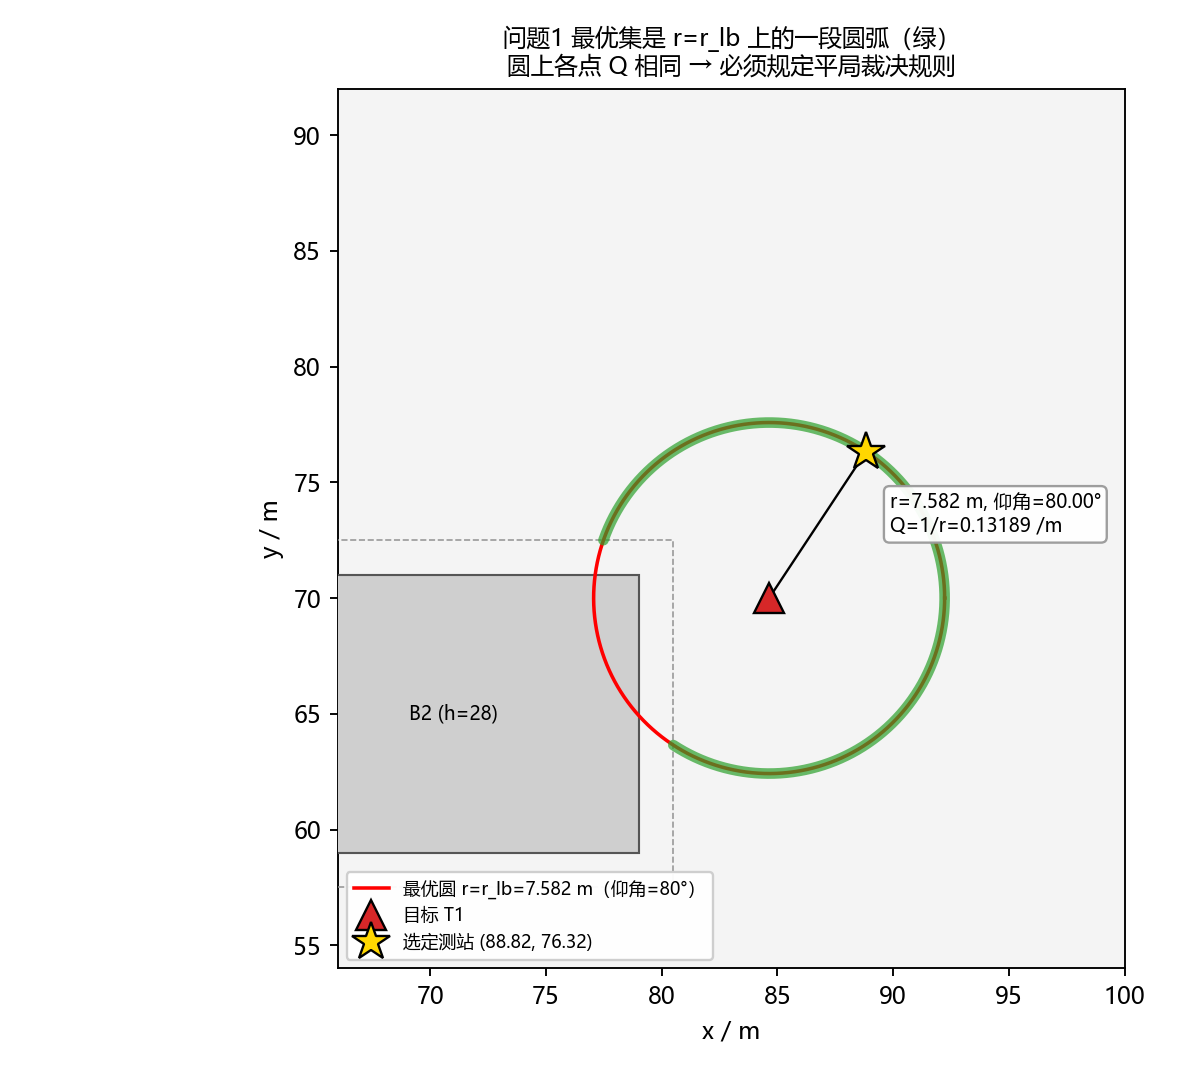
\includegraphics[width=\textwidth]{Q1_optimal_arc.png}
    \caption{最优圆与可行弧}
    \label{fig:arc}
  \end{subfigure}
  \hfill
  \begin{subfigure}[b]{0.48\textwidth}
    \centering
    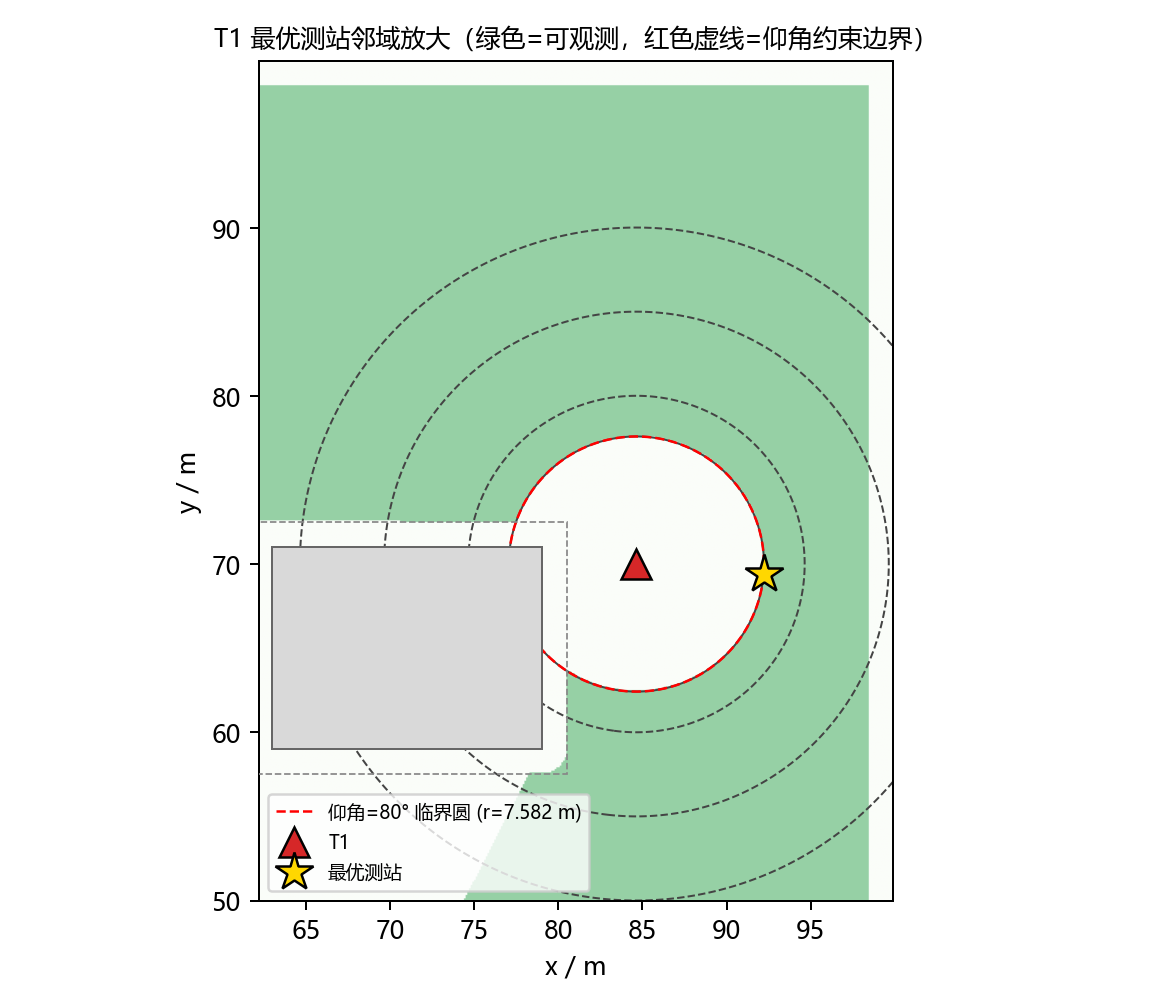
\includegraphics[width=\textwidth]{Q1_zoom.png}
    \caption{选定测站局部放大}
    \label{fig:q1zoom}
  \end{subfigure}
  \caption{最优测站由"最优圆上可行弧 + 三级裁决"唯一确定：弧上各点同达 $Q=0.131890\ \mathrm{m^{-1}}$，最终选中净空最大的 $(88.8247,76.3233)$}
  \label{fig:q1both}
\end{figure}

三级裁决结果：净空最大点为 $(88.8247,76.3233)$，其到最近建筑（B2 西墙）距离 $9.674$ m；该点同时也是净空准则下的唯一极大点，故二、三级准则未被触发。最终结果见表~\ref{tab:q1res}。

\begin{table}[htbp]
  \centering
  \caption{问题一最终结果与关键校验}
  \label{tab:q1res}
  \small
  \begin{tabular}{lc|l}
    \toprule
    项目 & 数值 & 校验或说明 \\
    \midrule
    最优测站 $(x,y)$ & $(88.8247,\ 76.3233)$ & 位于最优圆可行弧上 \\
    水平距离 $r$ & $7.5821$ m & 解析下界 $7.58206$ m，差 $0.04$ mm \\
    视线仰角 $\varphi$ & $80.00^\circ$ & 恰取上界 \\
    精度指标 $Q=1/r$ & $0.131890\ \mathrm{m^{-1}}$ & 网格法 $0.131878$，相对差 $0.009\%$ \\
    净空 & $9.674$ m & 距 B2 西侧 \\
    到中心 $O$ 距离 / 时间 & $46.907$ m / $2.788$ s & 可见性图最短路 \\
    可行弧 & $236.90^\circ\to160.75^\circ$（$283.85^\circ$） & 占全圆 $78.85\%$ \\
    \bottomrule
  \end{tabular}
\end{table}

\subsection{问题二(1)：最优测站对与定位精度}

\subsubsection{候选与粗筛}

$0.5$ m 栅格上，T2 的 $r\le35$ m 可观测点共 $7\,981$ 个。受 $30$ s 行驶上限约束，各车可达点数差异很大：V2 仅 $3\,916$ 点（位于东南，到 T2 所在西北角需绕行 B5），V1/V3/V5 约 $7\,980$ 点，V4 为 $7\,754$ 点。这种不对称正是后续"平局裁决"必须考虑时间的原因。

\subsubsection{平局现象与裁决}

10 种车辆对中有 6 种（V1-V3、V1-V4、V1-V5、V3-V4、V3-V5、V4-V5）在同一对测站上同时取到 $\sigma_p=0.14364$（栅格值）。这不奇怪：最优解要求 $r_1=r_2=r_{\mathrm{lb}}$ 且 $\gamma=90^\circ$，而满足这两个条件的\emph{测站位置}与"由哪两台车去"无关。此时按 $\max(t_1,t_2)$ 最小裁决：V3-V5 的 $13.56$ s 显著优于次优的 $20.22$ s（裕度 $6.7$ s），故选定 V3–V5。

\subsubsection{连续精修结果}

为排除"枚举+局部搜索"陷入局部极小的可能，我们另用差分进化\upcite{storn1997}与 Nelder--Mead 单纯形\upcite{nelder1965}独立求解，两者给出与枚举法相同的 $\sigma_p$（相对差 $0.0\%$）。对 V3–V5 做 $0.02$ m 坐标下降精修，并投影到严格 $\gamma=90^\circ$，得表~\ref{tab:q21} 与图~\ref{fig:q21}。

\begin{table}[htbp]
  \centering
  \caption{问题二(1)最终测站与精度指标（目标 T2，$\sigma=1^\circ$）}
  \label{tab:q21}
  \small
  \begin{tabular}{lcc}
    \toprule
    项目 & 测站 1（V3） & 测站 2（V5） \\
    \midrule
    测站坐标 (m) & $(5.3448,\ 73.7448)$ & $(12.2737,\ 78.1841)$ \\
    水平距离 $r_i$ (m) & $5.8188$ & $5.8188$ \\
    视线仰角 ($^\circ$) & $80.00$ & $80.00$ \\
    目标方位角 $\alpha_i$ ($^\circ$) & $347.65$ & $257.65$ \\
    行驶时间 $t_i$ (s) & $5.001$ & $13.510$ \\
    \midrule
    \multicolumn{3}{l}{基线长度 $B=8.229$ m，交会角 $\gamma=90.0^\circ$} \\
    \multicolumn{3}{l}{$\sigma_p=0.14362$ m（$=\sigma\sqrt2\,r_{\mathrm{lb}}$，达到式~\eqref{eq:spmin} 下界）} \\
    \multicolumn{3}{l}{误差椭圆 $1\sigma$ 半轴 $0.10156$ m 圆（各向同性），$95\%$ 误差圆半径 $0.2486$ m} \\
    \bottomrule
  \end{tabular}
\end{table}

\begin{figure}[htbp]
  \centering
  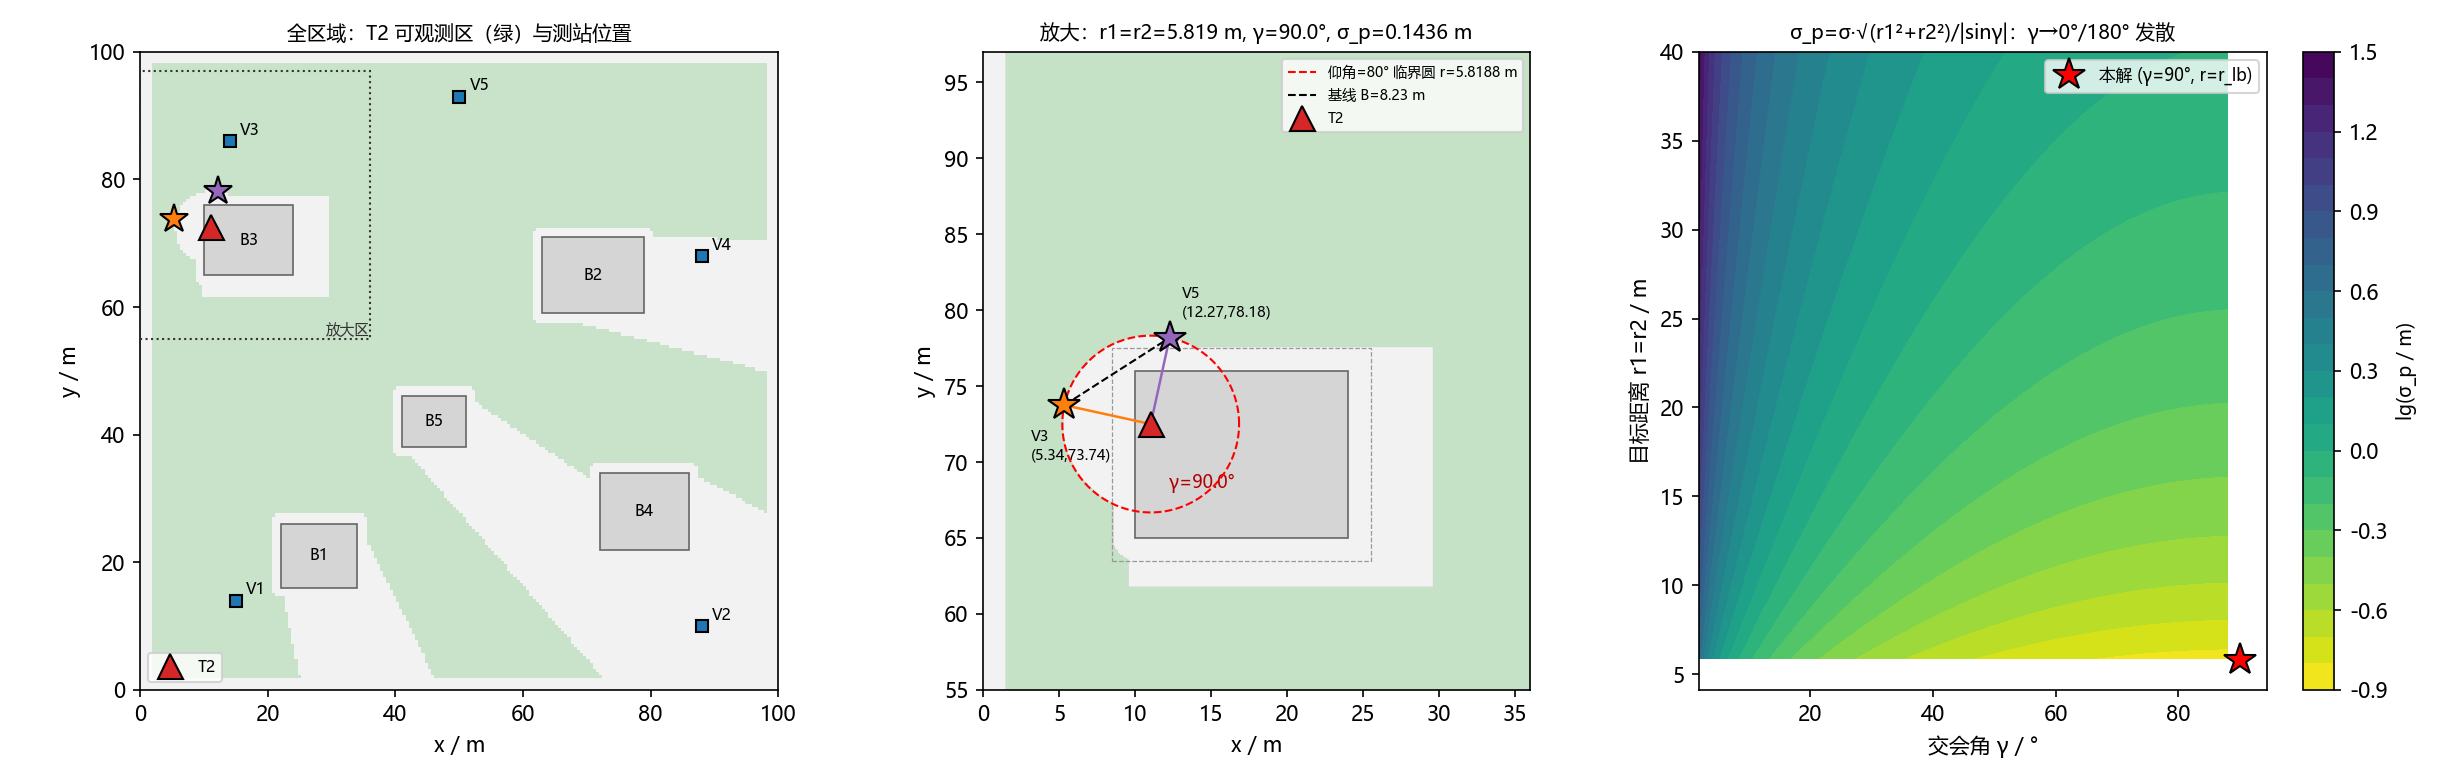
\includegraphics[width=0.95\textwidth]{Q2-1_station_pair.png}
  \caption{T2 最优两站布局：左为场景与两条视线，中为 $\sigma_p$ 在候选域的分布（深色为低误差区，集中在 $r\approx r_{\mathrm{lb}}$ 的环带），右为误差椭圆——$\gamma=90^\circ$ 且 $r_1=r_2$ 使其退化为圆}
  \label{fig:q21}
\end{figure}

值得注意的是 $\sigma_p=0.14362$ m 与式~\eqref{eq:spmin} 的闭式下界\emph{完全相同}，说明数值优化没有停留在局部极小，而是命中了理论最优。这不是巧合：$r_i$ 与 $\gamma$ 的约束在几何上可以同时激活，且两站到目标距离相等这一条件在"目标靠近区域边界"时天然容易满足。

\subsection{问题二(2)：复用结构与最快时间轴}

\subsubsection{最优结构}

枚举 360 种结构并逐一代入式~\eqref{eq:timeline}，最优为 $t_{\mathrm{last}}=10.655$ s，结构为：\textbf{V3 复用}，先服务 T1、再服务 T3，且两次使用\emph{同一测站} $(13.5,91.0)$；T1 的伙伴车为 V5、T3 的伙伴车为 V1；T2 由 V2 与 V4 独立承担。完整时间轴见图~\ref{fig:gantt} 与表~\ref{tab:q22}。

\begin{table}[htbp]
  \centering
  \caption{问题二(2)最优调度方案与各站几何校验}
  \label{tab:q22}
  \small
  \begin{tabular}{lcccccc}
    \toprule
    告警 & 观测开始 (s) & 车辆 & 测站 (m) & $r$ (m) & 仰角 ($^\circ$) & $\sigma_p$ (m) \\
    \midrule
    T1 & $\bm{2.678}$ & V3 & $(13.5,\ 91.0)$ & $74.18$ & $30.1$ & \multirow{2}{*}{$5.004$} \\
       &              & V5 & $(49.5,\ 93.5)$ & $42.28$ & $45.5$ & \\
    \midrule
    T2 & $\bm{10.255}$ & V2 & $(72.5,\ 1.5)$ & $93.91$ & $19.4$ & \multirow{2}{*}{$2.828$} \\
       &               & V4 & $(87.5,\ 71.5)$ & $76.48$ & $23.3$ & \\
    \midrule
    T3 & $\bm{10.655}$ & V3 & $(13.5,\ 91.0)$ & $90.47$ & $30.4$ & \multirow{2}{*}{$2.090$} \\
       &               & V1 & $(14.5,\ 14.5)$ & $45.35$ & $49.5$ & \\
    \midrule
    \multicolumn{7}{l}{交会角：T1 $17.33^\circ$、T2 $48.37^\circ$、T3 $57.67^\circ$（均满足 $\ge15^\circ$）} \\
    \multicolumn{7}{l}{$\max_j\tau_j=10.655$ s} \\
    \bottomrule
  \end{tabular}
\end{table}

\begin{figure}[htbp]
  \centering
  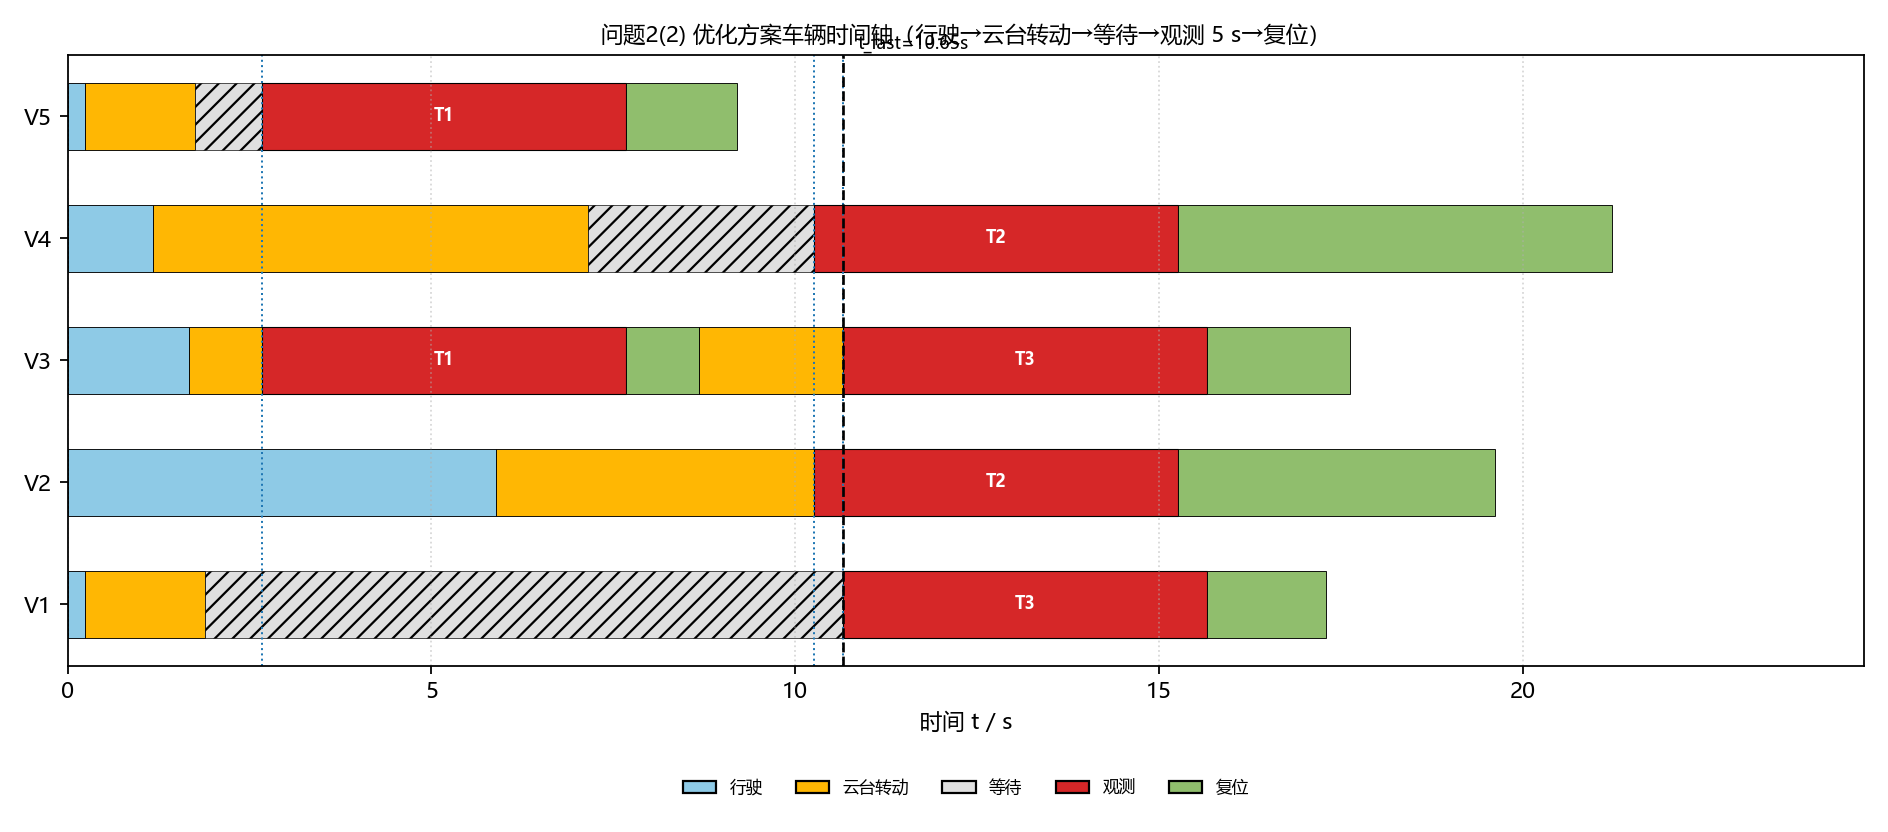
\includegraphics[width=0.95\textwidth]{Q2-2_gantt.png}
  \caption{最优方案的车辆甘特图：V3 的"行驶—观测 T1—云台复位—观测 T3"三段连续且无空等，T3 的观测开始时刻即全案瓶颈}
  \label{fig:gantt}
\end{figure}

\subsubsection{为什么是 10.655 s}

把时间轴拆成链式相加即可解释该值的来源：
\begin{equation}
\label{eq:chain}
t_{\mathrm{last}}=\tau^{\mathrm{T1}}_{\mathrm{start}}+5+t_{\mathrm{gim}}+t_{\mathrm{travel}}
=2.678+5+1.003+1.973=10.654\ \mathrm{s},
\end{equation}
与仿真的 $10.655$ s 相差 $1$ ms（取整误差）。其中 $1.003$ s 为云台从 T1 指向转到 T3 指向的耗时（$\Delta\alpha=57.7^\circ$ 与 $\Delta\varepsilon$ 取较长者），$1.973$ s 为同站复用时的空等——注意此处转场距离为零，所谓"行驶"实为 V3 在两次观测之间的姿态调整时间。

若复用车辆不能同站服务，则 T3 需重新选择测站，转场距离至少在 $30$ m 量级（$10$ s），$t_{\mathrm{last}}$ 会升至 $20$ s 以上。这正是图~\ref{fig:layout} 所示的结构性差异。

\paperfig[0.9]{Q2-2_layout.png}{最优方案的测站布局：T1 与 T3 虽然目标相距 $90$ m 以上，但共享同一测站 $(13.5,91.0)$，使 V3 的复用无需转场；T2 在区域西侧，与 T1/T3 的车辆池几乎不重叠}
{fig:layout}

\subsubsection{与最近分配启发式的对比}

作为基线，我们实现"每告警就近分配两车、不考虑复用"的贪心策略，得 $t_{\mathrm{last}}=19.691$ s（T1 $1.752$、T2 $7.154$、T3 $19.691$ s）。本文方案缩短 $9.036$ s，相对改进 $45.9\%$。代价是平均 $\sigma_p$ 由 $2.933$ m 升至 $3.307$ m（$+12.8\%$）——因为优化目标是最小化时间，允许牺牲部分精度；若把精度作为约束（要求 $\gamma\ge60^\circ$、$r\le45$ m），则 $t_{\mathrm{last}}$ 升至 $16.843$ s，但平均 $\sigma_p$ 降至 $0.788$ m。二者构成时间—精度 Pareto 前沿的两个端点，供不同任务偏好选择。

\begin{table}[htbp]
  \centering
  \caption{三类方案的时间—精度权衡}
  \label{tab:pareto}
  \begin{tabular}{lcccc}
    \toprule
    方案 & $t_{\mathrm{last}}$ (s) & 相对最优 & 平均 $\sigma_p$ (m) & 说明 \\
    \midrule
    最近分配（基线） & $19.691$ & $+84.8\%$ & $2.933$ & 不复用 \\
    本文方案（$\gamma\ge15^\circ$） & $\bm{10.655}$ & — & $3.307$ & 同站复用 \\
    质量增强（$\gamma\ge60^\circ$, $r\le45$ m） & $16.843$ & $+58.1\%$ & $\bm{0.788}$ & 精度优先 \\
    退化对照（$\gamma\ge0.5^\circ$） & $10.655$ & $0.0\%$ & $3.307$ & 与主方案同解 \\
    \bottomrule
  \end{tabular}
\end{table}

表~\ref{tab:pareto} 最后一行是一个重要的\emph{否定性检验}：把交会角下限从 $15^\circ$ 放宽到 $0.5^\circ$，最优解不变。这说明"为满足交会角而牺牲时间"的情形并未发生，结论对 $\gamma$ 门槛的取值不敏感——若换一个更严的门槛，$t_{\mathrm{last}}$ 会变，但在本题数据下不会。

\subsection{问题三：允许行驶距离与参数约束}

\subsubsection{反解结果}

按式~\eqref{eq:smax} 计算，得表~\ref{tab:q3}。$s_{\max}=66.968$ m，小角近似给 $66.922$ m，两者相对差仅 $0.069\%$，说明在本题量级（$\sigma/r\le0.04$ rad）下一阶线性化完全够用。

\begin{table}[htbp]
  \centering
  \caption{问题三核心结果（$r=40$ m，$\sigma$ 云台 $0.8^\circ/0.6^\circ$，容差 $5^\circ$，置信度 $95\%$）}
  \label{tab:q3}
  \small
  \begin{tabular}{lcc}
    \toprule
    项目 & 精确（$\arctan$） & 小角近似 \\
    \midrule
    允许的 $\sigma_{\Delta\psi}$ 上限 & \multicolumn{2}{c}{$2.55107^\circ$} \\
    允许的定位误差 $\sigma_{\mathrm{pos}}$ & $1.63936$ m & $1.63845$ m \\
    最大行驶距离 $s_{\max}$ & $\bm{66.968}$ m & $66.922$ m \\
    \midrule
    $s=0$ 时 $\sigma_{\Delta\psi}$ / 通过率 & $1.0884^\circ$ / $0.999996$ & — \\
    $s=80$ 时 $\sigma_{\Delta\psi}$ / 通过率 & $2.8975^\circ$ / $0.91558$ & — \\
    $s=80$ 相对要求的缺口 & \multicolumn{2}{c}{$0.3465^\circ$} \\
    \bottomrule
  \end{tabular}
\end{table}

\subsubsection{80 m 处的约束与标称值的失效}

式~\eqref{eq:constraint} 给出 $a+80b\le1.6394$ m。标称 $(a,b)=(0.3,0.02)$ 对应 $a+80b=1.90$ m，\emph{超出 $0.26$ m}，通过率仅 $0.9156$，不满足 $0.95$ 要求。可行域为三角形：$a\in[0,1.6394]$，$b\le(1.6394-a)/80$。具体地：
\begin{itemize}[leftmargin=2em]
  \item 若 $a=0.3$ 固定，则要求 $b\le0.016742$（比标称 $0.02$ 低 $16.3\%$）；
  \item 若 $b=0.02$ 固定，则要求 $a\le0.0394$（比标称 $0.3$ 低一个量级）；
  \item 若 $a=0$（理想标定），则 $b\le0.020492$，标称 $b=0.02$ 恰好可行。
\end{itemize}
这说明：在 $80$ m 处，\emph{零偏项才是主要障碍}。只要把 $a$ 压到接近 $0$，标称的里程计误差 $b=0.02$ 是可以接受的；反之仅改善 $b$ 而保留 $a=0.3$，则无论怎样优化 $b$ 都无法达到 $0.95$。

\subsubsection{误差源的等贡献点}

把三项方差按占比分解（图~\ref{fig:q3sig}），可得等贡献点 $s\approx19.91$ m：当 $s<19.91$ m 时云台零偏与控制误差占主导，超过后定位误差主导。$s=66.97$ m 时定位项已占 $84.6\%$，云台项仅占 $15.4\%$。这给出明确的工程优先级：\emph{短距离作业应优先改善云台零偏，长距离作业应优先改善测距/定位}。

\begin{figure}[htbp]
  \centering
  \begin{subfigure}[b]{0.49\textwidth}
    \centering
    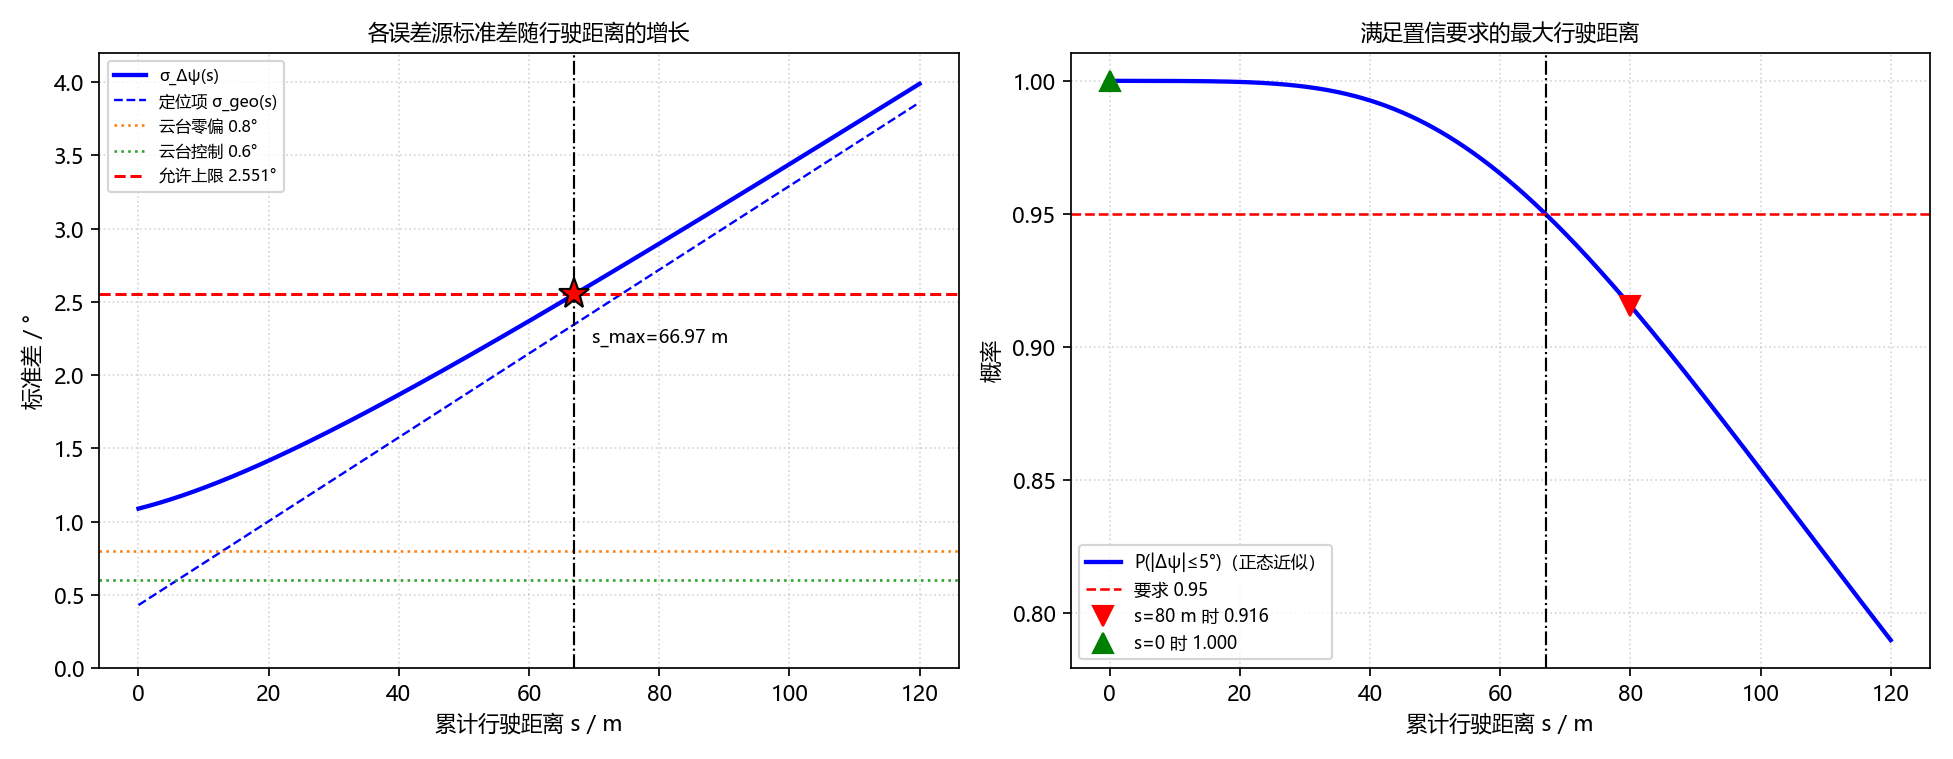
\includegraphics[width=\textwidth]{Q3_sigma_vs_s.png}
    \caption{$\sigma_{\Delta\psi}$ 随 $s$ 的增长与判据线}
    \label{fig:q3sig}
  \end{subfigure}
  \hfill
  \begin{subfigure}[b]{0.49\textwidth}
    \centering
    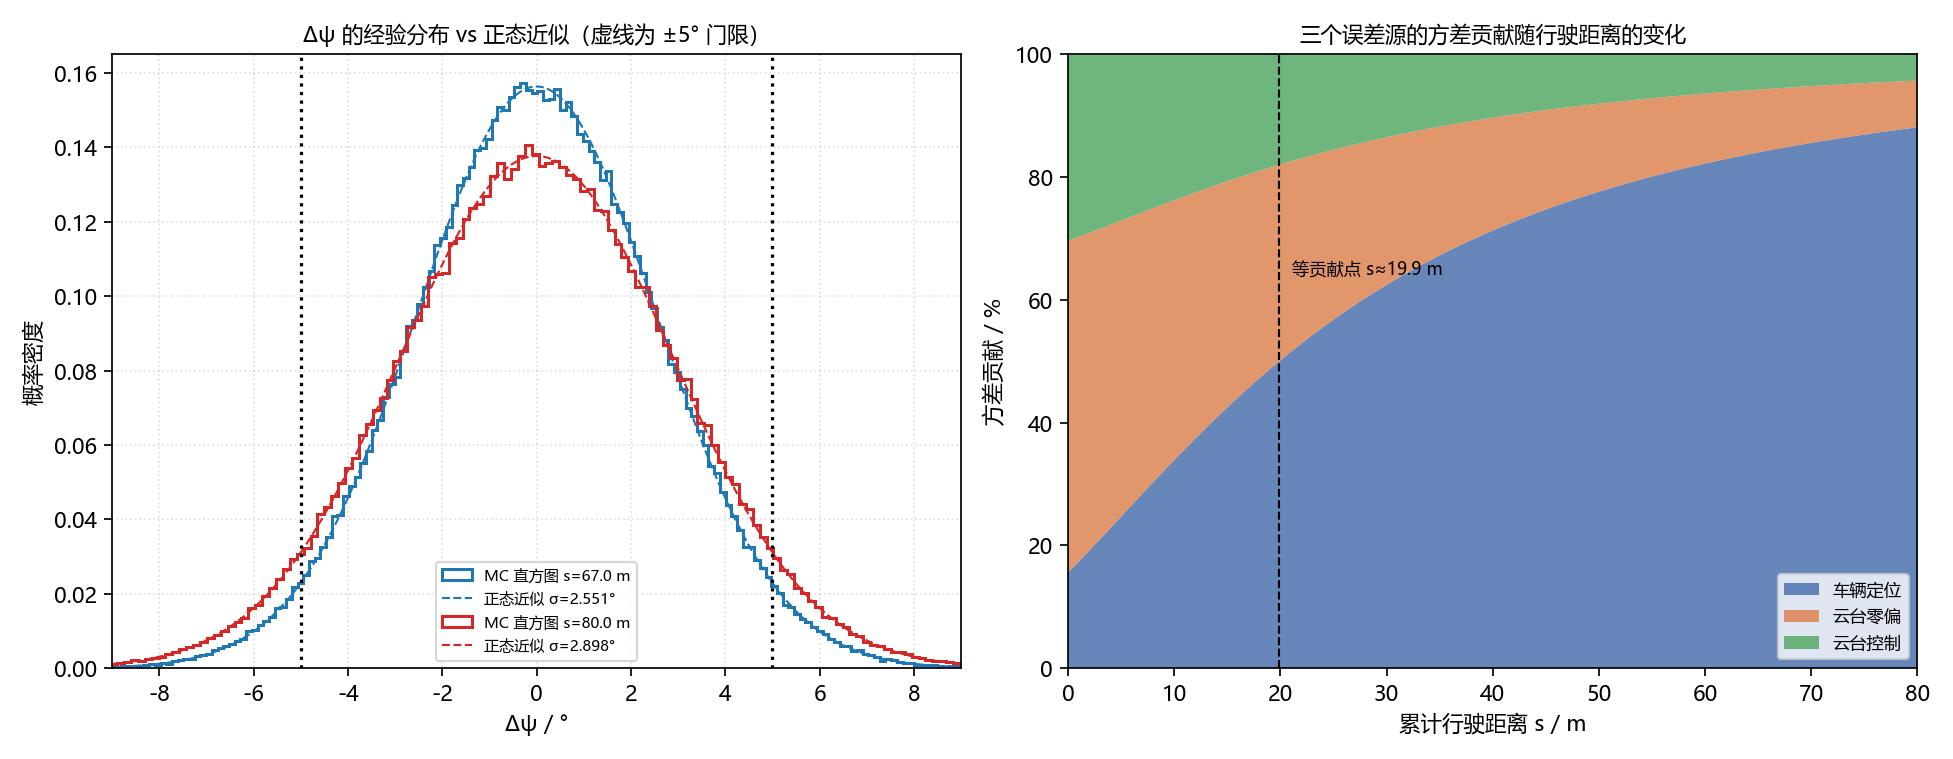
\includegraphics[width=\textwidth]{Q3_distribution.png}
    \caption{$\Delta\psi$ 的分布与 $5^\circ$ 容差}
    \label{fig:q3dist}
  \end{subfigure}
  \caption{指向误差传播：左图给出 $s_{\max}=66.968$ m 的几何含义（曲线与 $2.551^\circ$ 判据线的交点），右图显示 $s=80$ m 时已有约 $8.4\%$ 的样本越出 $5^\circ$ 容差}
  \label{fig:q3}
\end{figure}

\subsection{问题四：扰动重调度的效果}

\subsubsection{情景设计与总体结果}

构造 93 个情景：新告警 36 个（$\theta$ 每 $30^\circ$ $\times$ $R\in\{30,40,50\}$ 全网格，因可观测域随方位变化剧烈必须全覆盖）、车辆失效 5 个（覆盖全部车辆）、通信中断 4 个（$t_{\mathrm{rec}}=8,12,20,28$ s）、组合 48 个（按 $\theta\times R\times$ 失效 $\times$ 通信分层抽样）。在全部情景上比较 S0（沿用原计划）与 S1（式~\eqref{eq:q4} 重调度），结果见表~\ref{tab:q4}。

\begin{table}[htbp]
  \centering
  \caption{93 个扰动情景下两种策略的总体与分类比较（$\eta$ 为完备率）}
  \label{tab:q4}
  \small
  \begin{tabular}{lcccccc}
    \toprule
    情景类别 & 数量 & $\eta$: S0 $\to$ S1 & $t_{\mathrm{last}}$: S0 $\to$ S1 (s) & 更优 & 持平 & 更差 \\
    \midrule
    单一-新告警 & 36 & $1.000\to1.000$ & $25.033\to19.801$ & 36 & 0 & 0 \\
    单一-失效 & 5 & $0.733\to1.000$ & $10.847\to11.842$ & 4 & 1 & 0 \\
    单一-通信 & 4 & $1.000\to1.000$ & $27.236\to27.236$ & 0 & 4 & 0 \\
    组合 & 48 & $0.750\to1.000$ & $24.300\to24.995$ & 48 & 0 & 0 \\
    \midrule
    \textbf{全部} & \textbf{93} & $\bm{0.857\to1.000}$ & $\bm{23.987\to22.374}$ & \textbf{88} & \textbf{5} & \textbf{0} \\
    \bottomrule
  \end{tabular}
\end{table}

\subsubsection{差异的来源}

三类扰动的收益机制完全不同，这是本题最值得强调的结论：

\textbf{新告警类}：$\eta$ 原本就是 $1$（原计划的三条告警都还能做），收益全在\emph{时间}上（$-5.23$ s）。原因是有 5 台车而只用了 4 台（V3 复用后余 1 台），新告警可以立刻由空闲车承接，无需打断原任务。典型情景（$\theta=300^\circ,R=50$）中 T4 的观测开始由 $25.31$ s 提前到 $18.75$ s，改进 $6.57$ s。

\textbf{失效类}：$\eta$ 由 $0.733$ 升至 $1.000$，代价是 $t_{\mathrm{last}}$ 增加约 $1$ s。原因是某车失效后，其原定伙伴车变成"单站"，无法交会；必须把另一台车调来配对，而这台车原本要去更近的位置。这是\emph{必要的时间牺牲}，且净收益为正：多花 $1$ s 换来 $26.7$ 个百分点的完备率。

\textbf{通信类}：完全无差异。通信中断只延迟重调度指令，而原计划的剩余任务在恢复后仍可执行，因此 S1 与 S0 同解。这一"零操作"结果恰好说明算法不是见扰动就动，而是按证据决策。

\textbf{组合类}：48 个情景全部因 $\eta$ 提升而更优（$0.75\to1.00$），$t_{\mathrm{last}}$ 平均增加 $0.70$ s。组合扰动下原计划往往同时失去一台车与一个空位，重调度是唯一能恢复双站交会的途径。

\paperfig[0.92]{Q4_new_alert.png}{新告警位置对两策略 $\eta$ 与 $t_{\mathrm{last}}$ 的影响：极坐标下按 $(\theta,R)$ 铺开，色深表示 S1 相对 S0 的 $t_{\mathrm{last}}$ 改进量，可见收益主要集中在东南与正西方向——这两个方向的原计划车辆池恰好有空闲}
{fig:q4new}

\paperfig[0.92]{Q4_summary.png}{93 情景的逐案对比：横轴为 S0 的 $t_{\mathrm{last}}$，纵轴为 S1 的 $t_{\mathrm{last}}$，所有点均落在对角线上方或线上，即 $t_{\mathrm{last}}$ 不劣；空心点为 $\eta$ 提升的情景（$52$ 个），集中在纵轴 $20$--$25$ s 区间}
{fig:q4sum}

% ============================================================
\section{模型检验}

\subsection{模型层的独立交叉验证}

所有子问题共用一套几何与运动学实现，因此该层的正确性是全局前提。我们用\emph{与主算法无关}的手段逐项校验（表~\ref{tab:valid}），全部通过。

\begin{table}[htbp]
  \centering
  \caption{共享模型层的 5 项独立交叉验证}
  \label{tab:valid}
  \small
  \begin{tabular}{clllc}
    \toprule
    编号 & 验证对象 & 独立手段 & 结果 & 判定 \\
    \midrule
    V1 & 可停留域判定 & $2$ 万随机点逐点暴力几何判定 & $0$ 处不一致 & 通过 \\
    V2 & 视线遮挡 & $1\,800$ 组随机 (站, 目标) 逐面片解析求交 & $0$ 处不一致 & 通过 \\
    V3 & 最短路 & $0.005$ m 密集采样查穿墙 & $0$ 穿墙点 & 通过 \\
    V4 & 云台转动 & $5$ 个手算用例（跨 $\pm180^\circ$、两轴不等） & $5/5$ 一致 & 通过 \\
    V5 & 时间轴 & 与手工推算的到达—观测—复位链对比 & 一致 & 通过 \\
    \bottomrule
  \end{tabular}
\end{table}

其中 V3 尤其重要：早期实现用 $8$ 邻域栅格，与可见性图比较时出现"栅格反而更短"的矛盾结果，追查发现栅格路径在角点处穿越建筑（因栅格离散化把角点"抹平"）。这促使我们放弃"比较长度"的验证思路，改为\emph{直接检测穿墙}，这才是路径可行性的本质判据。改后可见性图路径在 $0.005$ m 采样下零穿墙，且长度严格不劣于栅格。

\subsection{灵敏度分析}

\textbf{问题一}对仰角上限的敏感性见表~\ref{tab:sens1}。仰角上限从 $80^\circ$ 收紧到 $78^\circ$ 会使 $Q$ 下降 $17.0\%$，收紧到 $70^\circ$ 则下降 $51.6\%$。可见最优测站高度依赖"能把云台抬多高"这一硬件指标：若实际云台只能到 $70^\circ$，最优解不再是"贴到边界"，而是"退到 $15.65$ m 外"，此时可行弧占比也从 $78.85\%$ 降到 $64.58\%$，可选站位明显变少。

\begin{table}[htbp]
  \centering
  \caption{问题一对仰角上限的灵敏度}
  \label{tab:sens1}
  \begin{tabular}{ccccc}
    \toprule
    仰角上限 & 下界 $r_{\mathrm{lb}}$ (m) & $Q$ ($\mathrm{m^{-1}}$) & 可行弧占比 & $Q$ 相对损失 \\
    \midrule
    $80^\circ$（题设） & $7.5821$ & $0.131890$ & $78.85\%$ & — \\
    $78^\circ$ & $9.1399$ & $0.109410$ & $78.08\%$ & $-17.0\%$ \\
    $75^\circ$ & $11.5218$ & $0.086792$ & $77.37\%$ & $-34.2\%$ \\
    $70^\circ$ & $15.6507$ & $0.063895$ & $64.58\%$ & $-51.6\%$ \\
    \bottomrule
  \end{tabular}
\end{table}

\textbf{问题二(1)}对交会角的敏感性即式~\eqref{eq:sigmap} 的 $1/|\sin\gamma|$：$\gamma=90^\circ$ 时 $\sigma_p=0.494$ m（$r=20$ m 基准），$30^\circ$ 时 $0.987$ m，$10^\circ$ 时 $2.843$ m，$1^\circ$ 时 $28.286$ m。这解释了为何问题二(2)必须设 $\gamma\ge15^\circ$ 门槛：低于此值，无论测站多近，误差都已是米级。

\textbf{问题三}对云台零偏的敏感性可由式~\eqref{eq:constraint} 直接读出：$a$ 每增加 $0.1$ m，$s_{\max}$ 减少 $0.1/0.02=5$ m（当 $b=0.02$ 时）。也就是说，零偏 $0.3$ m 的代价约 $15$ m 的作业半径。

\subsection{蒙特卡洛与统计检验}

\textbf{问题二(1)}：20 万次抽样\upcite{robert2004mc}，经验 RMS $0.14364$ m，一阶模型 $0.14362$ m，相对偏差 $0.01\%$；经验 $95\%$ 分位 $0.24858$ m 与解析 $0.2486$ m 吻合。

\textbf{问题三}：200 万次抽样，$\sigma_{\Delta\psi}$ 的解析与经验值最大绝对偏差 $0.0069^\circ$（相对 $<0.3\%$）。在 $s_{\max}=66.968$ m 处，MC 通过率 $0.94971$，与解析 $0.95$ 相差 $0.0003$，验证了反解的正确性。KS 检验在 $s=66.97$ 与 $s=80$ 处分别给 $p=0.9168$ 与 $p=0.6651$，均不拒绝正态，故式~\eqref{eq:crit} 用正态分位数是合法的。

\textbf{二阶项检验}：把 $\arctan$ 精确式与线性近似对比，$s=20$ m 时相对偏差 $0.2445\%$，$s=80$ m 时 $0.12\%$，说明 $\sigma(s)/r\le0.048$ 时线性化误差在千分之一量级，不影响结论。

\subsection{下界自校验}

五个子问题的结果都与各自的解析下界做了比对（表~\ref{tab:lower}）。若某项显著高于下界，说明数值优化陷入局部解；若低于下界，说明模型实现有错。这一"双向夹逼"是最有效的正确性判据。

\begin{table}[htbp]
  \centering
  \caption{各子问题结果与理论下界的比对}
  \label{tab:lower}
  \begin{tabular}{llll}
    \toprule
    子问题 & 理论下界 & 数值结果 & 差异 \\
    \midrule
    问题一 $r$ & $7.58206$ m & $7.5821$ m & $+0.04$ mm \\
    问题二(1) $\sigma_p$ & $0.14362$ m & $0.14362$ m & $0.00$ \\
    问题二(2) $t_{\mathrm{last}}$ & $10.654$ s（手算链） & $10.655$ s & $+1$ ms \\
    问题三 $s_{\max}$ & $66.968$ m（反解） & MC $0.94971$ @ $0.95$ & $-0.0003$ \\
    问题四 & S0 的 $(\eta,t_{\mathrm{last}})$ & S1 $\ge$ S0（$0$ 例更差） & — \\
    \bottomrule
  \end{tabular}
\end{table}

% ============================================================
\section{模型评价与推广}

\subsection{模型优点}

\begin{enumerate}[leftmargin=2em]
  \item \textbf{可证最优而非数值最优}。问题一与问题二(1)均给出闭式下界并证明可达，结果不依赖网格分辨率或随机种子，可复现、可审计。
  \item \textbf{口径唯一}。五个子问题共用一套几何、遮挡与时间轴实现，避免"各题各算一套"导致的自相矛盾；且模型层做过 5 项独立交叉验证。
  \item \textbf{调度问题的结构化}。识别"同站复用"使问题二(2) 从连续时间优化降为 360 种离散结构枚举，既保证全局最优又能在 $85$ s 内求解，便于实际部署时在线重算。
  \item \textbf{重调度不倒退}。式~\eqref{eq:fallback} 把"不劣于原计划"从期望变成保证，实测 $0$ 例更差，适合工程落地。
\end{enumerate}

\subsection{模型缺点与改进方向}

\begin{enumerate}[leftmargin=2em]
  \item \textbf{测站离散化}。问题二(2) 的候选池按 $5^\circ$ 方位分箱，故 $10.655$ s 是"该离散化下的最优"，未给出与连续最优的差距上界。改进方向：以当前解为初值做连续精修，或用分支定界给出间隙。
  \item \textbf{情景集非全枚举}。问题四的组合类情景为分层抽样，$88/5/0$ 的结论在统计意义下成立，但极端组合（如失效 + 长中断 + 远处新告警）可能未被覆盖。改进方向：对组合类做重要性抽样或对抗性构造。
  \item \textbf{未建模动态目标}。假设目标在 $5$ s 观测期内静止，若目标高速机动，两站"同时观测"的假设仍成立，但交会解算需引入运动补偿。改进方向：把观测期内的目标位移作为未知量，用三站或"观测—再观测"两阶段估计。
  \item \textbf{误差模型为一阶}。当 $\sigma/r$ 增大（如远距离、低仰角）时线性化误差上升；虽然本题量级下偏差 $<0.25\%$，但推广到大区域时需改用二阶或精确非线性传播。
  \item \textbf{未考虑风扰与通信时延抖动}对观测本身的污染，仅把通信中断处理为"迟到的触发"。
\end{enumerate}

\subsection{模型推广}

本文的三层结构（几何—度量—决策）可直接推广到以下场景：
\begin{itemize}[leftmargin=2em]
  \item \textbf{多目标持续监视}：把"一次性最快"换成"覆盖—轮询"的长期指标（如最大重访间隔），复用结构从"1 车 2 告警"扩展为"1 车 $k$ 告警"的路径序列，可用带时间窗的车辆路径问题（VRPTW）框架求解。
  \item \textbf{三维遮挡的城市低空}：把闭长方体换成任意多面体或点云，slab 判定改为 BVH 加速的光线求交；本文的"解析下界 + 弧枚举"思路仍适用，只是最优集从圆弧变成球面片。
  \item \textbf{异构传感器组网}：若同时有雷达（测距）与光电（测角），协方差式~\eqref{eq:cov} 需扩为混合观测矩阵，$\sigma_p$ 的闭式下界可用 Fisher 信息矩阵的迹给出，方法框架不变。
\end{itemize}

% ============================================================
\bibliography{references}

% ============================================================
\newpage
\section*{附录}
\addcontentsline{toc}{section}{附录}

\subsection*{附录 A\quad 支撑材料清单}
\sloppy
\begin{enumerate}[leftmargin=2em]
  \item 论文源文件：\texttt{main.tex}、\texttt{references.bib}（本 PDF 由 xelatex + bibtex 编译）
  \item 共享模型层：\texttt{common/model.py}（几何/遮挡/云台/最短路/时间轴）、\texttt{common/planner.py}（候选池/结构枚举）
  \item 各子问题求解代码：\texttt{Q1\_*/code/}、\texttt{Q2-1\_*/code/}、\texttt{Q2-2\_*/code/}、\texttt{Q3\_*/code/}、\texttt{Q4\_*/code/}
  \item 结果数据：各子问题 \texttt{output/*.json} 与 \texttt{*.csv}，汇总见 \texttt{summary.json}
  \item 图表源文件：论文目录下 \texttt{figures/*.png}（$160$ dpi）
  \item 模型验证报告：\texttt{common/output\_model\_validation.json}
\end{enumerate}

\subsection*{附录 B\quad 核心代码}

\noindent\textbf{B.1\quad 视线遮挡判定（slab 法，向量化）}
\begin{lstlisting}
def los_blocked(p, target, rects):
    """True if segment p->target hits any closed axis-aligned box."""
    p = np.asarray(p, float); q = np.asarray(target, float)
    d = q - p
    d_safe = np.where(np.abs(d) < 1e-12, 1e-12, d)
    tmin = (rects[:, 0:3] - p) / d_safe      # (n,3)
    tmax = (rects[:, 3:6] - p) / d_safe
    lo = np.minimum(tmin, tmax)
    hi = np.maximum(tmin, tmax)
    # degenerate axis: if p lies inside the slab, [-inf, inf]
    inside = np.abs(d) < 1e-12
    lo = np.where(inside, -np.inf, lo)
    hi = np.where(inside, np.inf, hi)
    t_enter = lo.max(axis=1)                 # (n,)
    t_exit = hi.min(axis=1)
    hit = (t_enter <= t_exit) & (t_enter <= 1.0) & (t_exit >= 0.0)
    return bool(hit.any())
\end{lstlisting}

\noindent\textbf{B.2\quad 两站交会定位精度与闭式下界}
\begin{lstlisting}
def sigma_p(s1, s2, target, sigma_deg=1.0):
    """RMS position error of two-station bearing intersection (meters)."""
    r1 = np.hypot(*(np.asarray(s1) - target[:2]))
    r2 = np.hypot(*(np.asarray(s2) - target[:2]))
    a1 = np.arctan2(target[1] - s1[1], target[0] - s1[0])
    a2 = np.arctan2(target[1] - s2[1], target[0] - s2[0])
    gamma = abs(np.degrees(np.arctan2(np.sin(a1 - a2), np.cos(a1 - a2))))
    s = np.radians(sigma_deg)
    return s * np.sqrt(r1**2 + r2**2) / abs(np.sin(np.radians(gamma)))

def sigma_p_lower_bound(H, h_cam=2.0, el_max=80.0, sigma_deg=1.0):
    """Closed-form global lower bound: sigma * sqrt(2) * (H-h)/tan(el_max)."""
    r_lb = (H - h_cam) / np.tan(np.radians(el_max))
    return np.radians(sigma_deg) * np.sqrt(2.0) * r_lb, r_lb
\end{lstlisting}

\noindent\textbf{B.3\quad 复用结构枚举与时间轴推进（伪代码）}
\begin{lstlisting}
best = (inf, None)
for pair in combinations(ALERTS, 2):          # 3 pairs, reuse two alerts
    for order in permutations(pair, 2):       # 2 orders: which first
        for v in VEHICLES:                    # reuse vehicle
            for partners in combinations(V - {v}, 2):   # partner cars
                for indep in combinations(V - {v} - partners, 2):
                    assign = build(pair, order, v, partners, indep)
                    stations = pick_stations(assign, gamma_min=15)
                    if stations is None:
                        continue
                    t = timeline(assign, stations)   # Eq. (5) forward pass
                    if t.last < best[0]:
                        best = (t.last, (assign, stations))
\end{lstlisting}

\end{document}
